\chapter{Linear Collider Concepts}
\section{Main Parts of a linear collider}
The current two main linear accelerator projects, the International Linear Collider (ILC)\cite{ILCdes} and the Compact Linear Collider (CLIC)\cite{CLICdes}, are composed by similar main parts:\par
\begin{itemize}
 \item \textbf{Electron and Positron Sources:} is a laser driven photo-injector. The photons illuminate a GaAs cathode producing an electron current.\par
 Positrons are produced by electrons guided through a helical undulator. The photons illuminate a target to produce $e^-e^+$ pairs. The positrons are selected by deviating their trajectory with a magnet.\par
 \item \textbf{Damping Rings:} The pre-accelerated electron and positron beams are injected into the damping rings, composed of superconducting wigglers,  to make the beam radiate thus reducing the beam emittances to reach the small beam sizes in the collision.
 \item \textbf{Main Linac:} After the emittance reduction the beam passes through a chain of accelerating structures to increase the particles energy up to the design value while preserving as best as possible the normalized emittance.
 \item \textbf{Beam Delivery System (BDS):} is the beam transport system from the linac acceleration section to the collision at the IP. Its main purpose is the beam diagnose and collimation, and also the beam size reduction in a subsection called Final Focus Section~(FFS).\par
 The main purpose of this work is related to the FFS and the IP region, thus, it will be explained in detail in the following sections.\par
\end{itemize} 
\section{The Final Focus Section (FFS)}
In the Final Focus Section (FFS) the goal is to minimize the beam size. If the lattice is conceived as a telescope where the matrix elements are as in Eq.~(\ref{eq:telescope}), being $M_x, M_y$ the magnifications in horizontal and vertical planes, then, beam size to the first order does not depends on the beam energy spread $\delta$. Considering the second and third order components in the transfer map, as in Eq.~(\ref{eq:tmap}), then, the telescope properties show that the main contribution to beam size is chromaticity $\xi_{x\atop y}$ given by the elements $T_{126},$ and $T_{346}$~\cite{Brown:1987}, identified in~\cite{GarciaMorales:1982827} as
\begin{equation}
 \xi_x = \frac{1}{\beta_x^*}\left(T_{116}^2\beta_{x0}+T_{126}^2\frac{1}{\beta_{x0}}\right)\qquad
 \xi_y = \frac{1}{\beta_y^*}\left(T_{336}^2\beta_{y0}+T_{346}^2\frac{1}{\beta_{y0}}\right)
\end{equation}
being the 0-index the values at the input and *-index the values at the output. For this reason, the FFS has been conceived as a telescope to demagnify the beam size with minimum effect of energy spread, where the main issue is the large chromaticity generated at the Final Doublet (FD), the last pair of quadrupoles which focus the beam at the Interaction Point (IP).
\begin{equation}
R=
 \begin{pmatrix}
   M_x & 0 & 0 & 0 \\
   0 & 1/M_x & 0 & 0 \\
   0 & 0 & M_y & 0 \\
   0 & 0 & 0 & 1/M_y \\
  \end{pmatrix}\label{eq:telescope}
\end{equation}
\begin{equation}
x_i=\sum_{j=1}^6R_{ij}x_j+\sum_{j,k=1}^6T_{ijk}x_jx_k+\sum_{j,k,l=1}^6U_{ijkl}x_jx_kx_l+\cdots\qquad x_i\in x,x',y,y',\tau,\delta\label{eq:tmap}
\end{equation}
\section{Overview of FFS effects}
\subsection{Chromaticity}
As in the case of light beams through lenses, the longitudinal focal point location depends on the beam energy spread. This effect is called chromaticity.  Figure~\ref{f:chrom} represents schematically the focusing effect of a magnet as a lens. A particle with the design momentum crossing the lens at a distance $y_0$ from the center will be focused at $l^*$. Off-momentum particles with higher or lower momentum will be under-focused or over-focused, respectively. This produces a variation in the transverse position at the focal distance $l^*$ increasing the beam size.\par
\begin{figure}[!hbt]
\centering
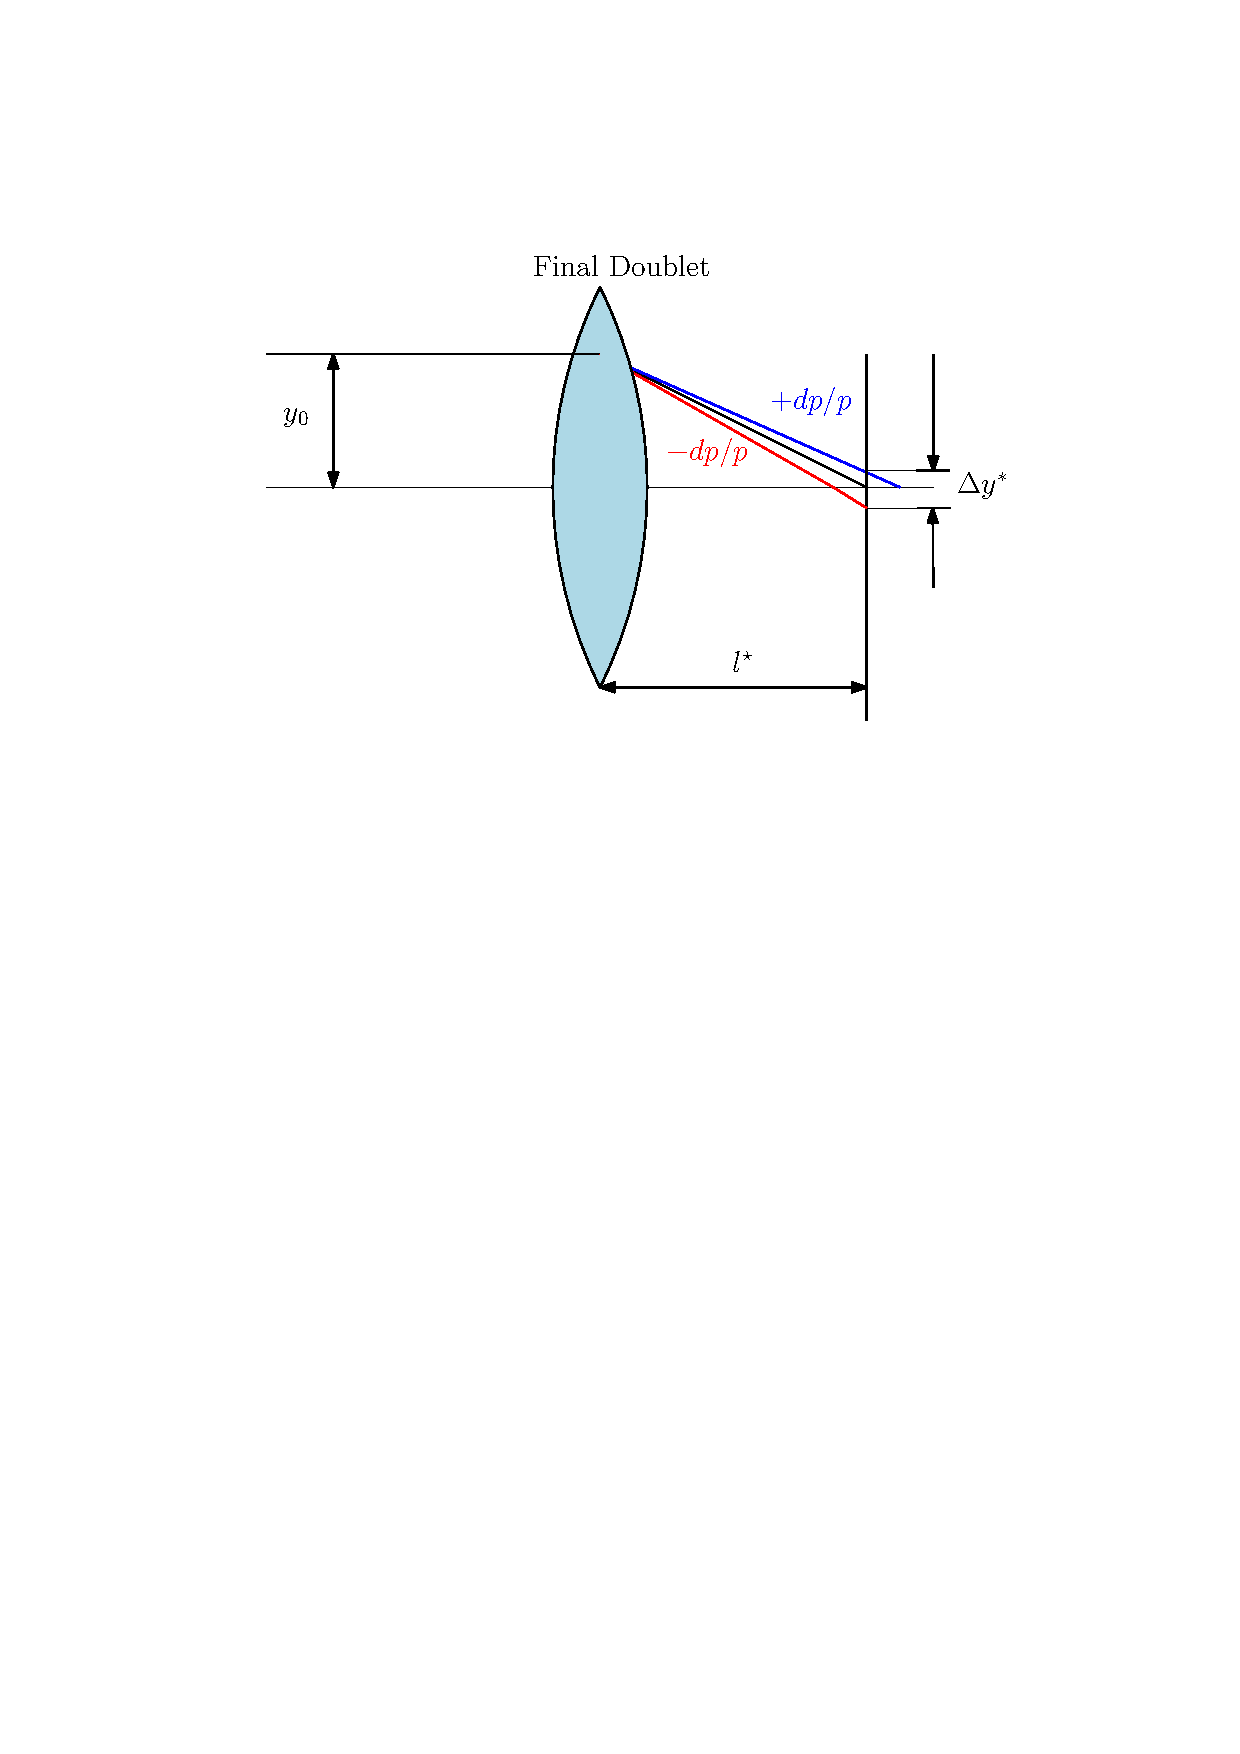
\includegraphics[scale=0.5]{chromaticity.pdf}\caption{Chromaticity. Particles with off-momentum energy are focused at different longitudinal locations increasing the beam size.}\label{f:chrom}
\end{figure}
The effect on the beam size is commonly estimated as
\begin{equation}
 \frac{\Delta y^*_{rms}}{\sigma^*_y}\approx\frac{l^*}{\beta^*}\sigma_\delta\approx\xi_y\sigma_\delta
\end{equation}
where $l^*$ is the focal length, $\sigma_\delta$ is the second moment of the energy spread distribution, $\beta_y^*$ is the optical $\beta$ function at the focal position and $\xi_y$ is the chromaticity.\par
The chromatic dilution of the beam size can be expressed as 
\begin{equation}
 \sigma^*_y\approx\sigma_{y,0}\sqrt{1+\xi_y^2\sigma^2_\delta}
\end{equation}
where $\sigma_{y,0}$ is the transverse beam size with zero energy spread.\par
An study of chromaticity minimum chromaticity generation in the FD is presented in Section~\ref{s:chromFD}.
\subsubsection{Chromaticity correction}\label{s:chromcorr}
In the thin lens approximation with a vertically focusing quadrupole magnet of thickness $ds$, the kick in angle given to a crossing particle is expressed in \cite{CAS9104} as
\begin{equation}
 dx'=k_q(1-\delta)xds\qquad dy'=-k_q(1-\delta)yds
\end{equation}
where $dx', dy'$ are the horizontal and vertical angle kick respectively, $k_q$ is the quadrupole gradient and $\delta=dP/P_0$ is the energy spread. A combination of bending magnets and sextupoles is used to substract the extra kick due to energy spread.\par
First, horizontal position and energy are correlated by dispersion, $\eta_x$, generated by bending magnets \cite{CAS9104}. This divides the particle motion in two parts: the betatron motion and an offset equal to $\eta_x\delta$. Equation~(\ref{eq:coortrans}) shows the coordinate transformation.
\begin{align}
 x\rightarrow& x_\beta + \eta_x \delta\label{eq:coortrans}\\
 y\rightarrow& y_\beta\notag
\end{align}
Then, sextupoles are located in dispersive regions ($\eta_x\neq0$) to kick the particles cancelling the quadrupole angle kick dependence on $\delta$. The quadrupole and sextupoles kicks in dispersive region are in Eq.~(\ref{eq:sextkick}), where $k_s$ is sextupole gradient.
\begin{align}
 \text{Quadrupole:}&\qquad dx'=k_q(1-\delta)(x_\beta+\eta_x\delta)ds\qquad& dy'=&-k_q(1-\delta)y_\beta ds \label{eq:sextkick}\\
 \text{Sextupole:}&\qquad dx'=\frac{1}{2}k_s[(x_\beta+\eta_x\delta)^2+y_\beta^2]ds\qquad& dy'=&-k_s(x_\beta+\eta\delta)y_\beta ds\notag
\end{align}
The chromatic terms, $k_q x_\beta\delta$ and $k_q y_\beta\delta$, are cancelled by matching $k_q$ and $k_s\eta_x$.\par
The geometric terms introduced by the sextupole, $\frac{1}{2}~k_s(x^2_\beta+y^2_\beta)$ and $k_sx_\beta y_\beta$, are cancelled by another sextupole, both separated by a transport matrix equal to $-I$ transformation, being $I$ the identity transport matrix.\par
The remaining terms are cancelled by a combination of bending magnets and sextupoles location and strengths. Two methods have been develop to achieve the cancellation all second order terms: the non-local correction and the local correction. A third method has been recently introduced, called the non-interleaved correction.\par
%
\textbf{Non-local correction:}~The non-local correction scheme~\cite{Brown:1988} compensates upstream the chromaticity in the Final Doublet (FD). Figure~\ref{f-Non-local} shows schematically the lattice configuration, where QF1 and QD0 constitute the FD, B0 to B5 are dipole magnets to produce horizontal dispersion, SD and SF sextupoles are used to cancel vertical and horizontal chromaticity respectively.\par
The chromatic terms, $k_q x_\beta\delta$ and $k_q y_\beta\delta$, are cancelled by making $k_q=k_s\eta_x$.\par
The term $k_q\eta_x\delta$ disappears because the final doublet is in a non-dispersive region.\par
The second order dispersion generated by the sextupoles, $\frac{1}{2}k_s\eta_x\delta^2$, is cancelled by matching the dispersion and sextupole strengths in the $-I$ transformation.
\begin{figure}[h]
   \centering
   \includegraphics*[scale=0.2,angle=0]{nonlocalcorr2.pdf}
   \caption{Non-local chromaticity correction.}
   \label{f-Non-local}
\end{figure}\par
\textbf{Local correction:}~The local chromaticity correction scheme~\cite{Raimondi:2000} compensates chromaticity inside the FD and Fig.~\ref{f-local} shows the sextupoles locations.\par
The non-zero dispersion in the FD generates an offset on the quadrupole horizontal focusing center, $x=x_\beta+\eta_x\delta$.\par
The second order dispersion, $k_q\eta_x\delta^2$ and $\frac{1}{2}k_s\eta_x\delta^2$, is half cancelled if $k_q=k_s\eta_x$. One solution is to double the sextupole strength and produce the entire chromaticity upstream in a non-dispersive region.\par
\begin{figure}[!htb]
   \centering
   \includegraphics[scale=0.2,angle=0]{localcorr2.pdf}
   \caption{Local chromaticity correction.}
   \label{f-local}
\end{figure}
\textbf{Non-interleaved correction:} The non-interleaved correction scheme is presented in Section~\ref{s:noninterleaved}.
\subsection{Pinch effect and Beamstrahlung}\label{s:beastr}
The electric charge interaction between bunches when the two bunches cross one another at the IP produces focusing for opposite charges and defocusing when bunches are of the same charge. This is called pinch effect. The change of trajectory leads to a loss of energy of the particles, called beam strahlung~\cite{Schulte:331845}.\par
The pinch effect could be used to determine the beam-beam relative offset because of the change in angle of the out-going trajectory after the interaction~\cite{Bambade:1989pb}. On the other hand, although the focusing effect increases the luminosity for bunches with opposite charge, the energy spread generated by the interaction reduces luminosity. This requires to separate the luminosity in total luminosity and peak luminosity.\par
The peak luminosity only accounts for those interactions between particles with at least 99\% of the nominal energy, while total luminosity accounts interactions at all energies.\par
Linear colliders require to minimize the beam size at the IP of the two beams to increase luminosity while also limiting the energy loss due to beamstrahlung $\delta_{BS}$. Equation~\ref{eq:lum_rad} highlights the dependence with beam size in the tranversal planes, where $f_{rep}$ is the repetion frequency of the two particle bunches collision, $E$ is the beam energy, and $\sigma_x$ and $\sigma_y$ are the horizontal and vertical beam sizes.
\begin{equation}
 L \propto \frac{f_{rep}n_b^2}{\sigma_x\sigma_y}\qquad\delta_{BS}\propto\frac{n_b^2E}{(\sigma_x+\sigma_y)^2}\label{eq:lum_rad}
\end{equation}
Table~\ref{t:lum_rad} shows how the beam size is decreased in all current linear collider projects, introduced in Section \ref{s:lincoll}, to compensate lower repetition rate and charges. In addition, horizontal beam size is larger than vertical beam size to preserve luminosity while reducing the beam strahlung effect.\par
\begin{table}[h]
{%\scriptsize
\centering
\begin{tabular}{l||c|c|c}\hline
Parameter, Symbol, [Unit]& ILC & CLIC 500 GeV& CLIC 3 TeV\\\hline\hline
Energy/e$^-$, $E$ [TeV]& 0.250 & 0.250 & 1.500\\
Bunch population, $n_b$ &$2\times10^{10}$&$6.8\times10^9$&$3.72\times10^9$\\
Repetition rate, $f_{rep}$, [Hz]&5 &50&50\\
H/V. IP beam size, $\sigma_x/\sigma_y$, [nm] &474/5.9&202/2.3&40/1\\\hline
E loss (Beamstrahlung), $\delta_{BS}$, [$\Delta E/E$]&0.07&0.07&0.28\\
Luminosity, $L$, [cm$^{-2}\cdot$s$^{-1}$]&$1.57\times10^{34}$ & $2.3\times10^{34}$&$5.9\times10^{34}$\\\hline
\end{tabular}\caption{Luminosity and beamstrahlung for the three current linear collider projects.}\label{t:beam_rad}
}
\end{table}
% \begin{table}[h]
% {\scriptsize
% \centering
% \begin{tabular}{l|c||c|c|c|c}\hline
% Parameter & Symbol & LHC & ILC & CLIC 500 GeV& CLIC 3 TeV\\\hline\hline
% Energy/z (TeV) & $E$& 7& 0.250 & 0.250 & 1.500\\
% Bunch population & $n_b$ &$1.15\times10^{11}$&$2\times10^{10}$&$6.8\times10^9$&$3.72\times10^9$\\
% Repetition rate [Hz] &$f_{rep}$& $11.1\times10^{3}$&5 &50&50\\
% H/V. IP beam size [nm] & $\sigma_x/\sigma_y$&$16.6\times10^{3}$&474/5.9&202/2.3&40/1\\\hline
% % E loss (Beamstrahlung) [$\Delta E/E$] &$\delta_{BS}$&-???&0.07&0.07&0.28\\
% Luminosity &$L$& $10^{34}$ &$1.57\times10^{34}$ & $2.3\times10^{34}$&$5.9\times10^{34}$\\\hline
% \end{tabular}\caption{Luminosity and beamstrahlung for the three current linear collider projects.}\label{t:beam_rad}
% }
% \end{table}
\subsection{Crossing angle}
It is necessary to intruduce a crossing angle between the two beam lines to avoid the near encounters of the in-going and out-going bunches. For beams without pinch effect the effect on luminosity for a crossing angle $\alpha$ is given by \cite{Napoly:240071}
\begin{equation}
 \frac{L}{L_0}=\frac{1}{\sqrt{1+\left(\frac{\sigma_z}{\sigma_x}\tan\frac{\alpha}{2}\right)}}
\end{equation}
where $\sigma_z$ and $\sigma_x$ are the longitudinal and horizontal beam sizes. The luminosity can be restored by rotating the beam using a crab cavity \cite{PhysRevSTAB.16.041001}.
\subsection{Hourglass effect}
To consider the beam size constant along the whole collision length is some cases is not a good approximation because of the beam divergence due the strong focusing. In a low-$\beta$ region near the IP, the beam size is
\begin{equation}
 \sigma(s)=\sigma^*\sqrt{1+\left(\frac{s}{\beta^*}\right)^2}
\end{equation}
where $s$ is the longitudinal position centered in the IP, and $\sigma^*$ is the beam size at the IP. This is important because not all particles will collide with minimum transverse beam size along the bunch length $\sigma_z$, affecting the luminosity \cite{chao}. The optimum $\beta_y^*$ that maximizes the luminosity is $\beta_y^*\approx\sigma_z$.\par
\subsection{Synchrotron Radiation}
Synchrotron radiation in the FFS increases the beam size \cite{Sands} thus affecting the luminosity, and can form background in the detector~\cite{Schulte:331845}. The beam size contribution from synchrotron radiation is studied in Section~\ref{bendrad}. The photons contributing to background should be collimated before the reach the detector.\par
Synchrotron radiation in the FD is dangerouse because the photons can not be collimated in front of the detector. To avoid any hitting the first and second quadrupole in the opposite line one must collimate the beam to achieve safe beam size. The Synchrotron radiation in the FD also contributes to beam size, and it limits the minimum vertical size achievable. Section~\ref{s:Oideeffect} presents the effect of the closest quadrupole to the IP, QD0.\par
\subsection{Tolerances}
The FFS has very tight tolerances because of the small beam size at the IP. Magnet strengths, position and tilt yield imperfections contribute the beam size growth.\par
The tuning is the procedure which brings the system performance to its design values. Since the initial errors are unknown, the tuning requires a statistical study. Usually more than 100 machines with randomly distributed errors are considered in computer simulations. The simulated tuning reproduces a realistic tuning procedure in a machine~\cite{GarciaMorales:1982827,Minty:629879}.\par
